%%
%% Copyright 2022 OXFORD UNIVERSITY PRESS
%%
%% This file is part of the 'oup-authoring-template Bundle'.
%% ---------------------------------------------
%%
%% It may be distributed under the conditions of the LaTeX Project Public
%% License, either version 1.2 of this license or (at your option) any
%% later version.  The latest version of this license is in
%%    http://www.latex-project.org/lppl.txt
%% and version 1.2 or later is part of all distributions of LaTeX
%% version 1999/12/01 or later.
%%
%% The list of all files belonging to the 'oup-authoring-template Bundle' is
%% given in the file `manifest.txt'.
%%
%% Template article for OXFORD UNIVERSITY PRESS's document class `oup-authoring-template'
%% with bibliographic references
%%

%%%CONTEMPORARY%%%
%\documentclass[unnumsec,webpdf,contemporary,large]{oup-authoring-template}%
%\documentclass[unnumsec,webpdf,contemporary,large,namedate]{oup-authoring-template}% uncomment this line for author year citations and comment the above
%\documentclass[unnumsec,webpdf,contemporary,medium]{oup-authoring-template}
%\documentclass[unnumsec,webpdf,contemporary,small]{oup-authoring-template}

%%%MODERN%%%
%\documentclass[unnumsec,webpdf,modern,large]{oup-authoring-template}
\documentclass[unnumsec,webpdf,modern,large,namedate]{oup-authoring-template}% uncomment this line for author year citations and comment the above
%\documentclass[unnumsec,webpdf,modern,medium]{oup-authoring-template}
%\documentclass[unnumsec,webpdf,modern,small]{oup-authoring-template}

%%%TRADITIONAL%%%
%\documentclass[unnumsec,webpdf,traditional,large]{oup-authoring-template}
%\documentclass[unnumsec,webpdf,traditional,large,namedate]{oup-authoring-template}% uncomment this line for author year citations and comment the above
%\documentclass[unnumsec,namedate,webpdf,traditional,medium]{oup-authoring-template}
%\documentclass[namedate,webpdf,traditional,small]{oup-authoring-template}

%\onecolumn % for one column layouts

%\usepackage{showframe}
\usepackage{fontenc}
\graphicspath{{Fig/}}

\usepackage{minted}

% line numbers
%\usepackage[mathlines, switch]{lineno}
%\usepackage[right]{lineno}

\theoremstyle{thmstyleone}%
\newtheorem{theorem}{Theorem}%  meant for continuous numbers
%%\newtheorem{theorem}{Theorem}[section]% meant for sectionwise numbers
%% optional argument [theorem] produces theorem numbering sequence instead of independent numbers for Proposition
\newtheorem{proposition}[theorem]{Proposition}%
%%\newtheorem{proposition}{Proposition}% to get separate numbers for theorem and proposition etc.
\theoremstyle{thmstyletwo}%
\newtheorem{example}{Example}%
\newtheorem{remark}{Remark}%
\theoremstyle{thmstylethree}%
\newtheorem{definition}{Definition}

\begin{document}

\journaltitle{Bioinformatics}
\DOI{DOI HERE}
\copyrightyear{2023}
\pubyear{2019}
\access{Advance Access Publication Date: Day Month Year}
\appnotes{Paper}

\firstpage{1}

%\subtitle{Subject Section}

\title[tstrait]{tstrait: a quantitative trait simulator for ancestral recombination graphs}

\author[1,2,$\ast$]{Daiki Tagami\ORCID{0000-0002-0923-1070}}
\author[2]{Gertjan Bisschop\ORCID{0000-0001-8327-0142}}
\author[2]{Jerome Kelleher\ORCID{0000-0002-7894-5253}}

\authormark{D.Tagami et al.}

\address[1]{\orgdiv{Department of Statistics}, \orgname{University of Oxford}, \orgaddress{\street{24-29 St Giles'}, \postcode{Oxford OX1 3LB}, \country{United Kingdom}}}
\address[2]{\orgdiv{Big Data Institute, Li Ka Shing Centre for Health Information and Discovery}, \orgname{University of Oxford}, \orgaddress{\street{Old Road Campus}, \postcode{Oxford OX3 7LF}, \country{United Kingdom}}}

\corresp[$\ast$]{Corresponding author. \href{email:daiki.tagami@hertford.ox.ac.uk}{daiki.tagami@hertford.ox.ac.uk}}

\received{Date}{0}{Year}
\revised{Date}{0}{Year}
\accepted{Date}{0}{Year}

\abstract{
\textbf{Summary:} 
\texttt{tstrait} is a new open-source Python library that incorporates a wide range of state-of-the-art algorithms for simulating quantitative traits based on an ancestral recombination graph (ARG). ARG is an active field of research in population genetics and statistical genetics due to its promising aspects in genome-wide association study (GWAS), and this package serves as an essential infrastructure for utilizing ARG in GWAS simulations. In this work, we provide an overview of the simulation framework that is incorporated in \texttt{tstrait} and highlight some recent developments in ARG.\\
\textbf{Availability and Implementation:} \texttt{tstrait} is available as an open-source Python package. The full documentation with examples and workflow templates is available on \url{https://tskit.dev/tstrait/docs/}, and the development version is maintained on Github (\url{https://github.com/tskit-dev/tstrait}).\\
\textbf{Contact:} \href{daiki.tagami@hertford.ox.ac.uk}{daiki.tagami@hertford.ox.ac.uk}\\
}
%\abstract{Abstracts must be able to stand alone and so cannot contain %citations to
%the paper's references, equations, etc. An abstract must consist of a single
%paragraph and be concise. Because of online formatting, abstracts must appear
%as plain as possible.}
%\keywords{keyword1, Keyword2, Keyword3, Keyword4}

% \boxedtext{
% \begin{itemize}
% \item Key boxed text here.
% \item Key boxed text here.
% \item Key boxed text here.
% \end{itemize}}

\maketitle

\section{Introduction}

Genome-wide association study (GWAS) tests genetic variants across the entire genome of individuals to identify genetic variants that are statistically associated with a specific trait \citep{uffelmann2021}. GWAS has successfully identified many loci that are associated with various human diseases and traits \citep{ishigaki2022,locke2015,mahajan2022,mathieson2023,yengo2022}, and GWAS results have actively been used in human trials and clinical practices \citep{visscher2017}. In spite of its advantages, population structure and demographic histories can heavily influence GWAS results \citep{uffelmann2021}, so it would be necessary for researchers to implement these factors when conducting GWAS.

Ancestral recombination graphs (ARGs) have many promising aspects in GWAS. Recent studies have shown that genealogy-based association can detect more ultra rare variants than conventional methods \citep{zhang2023}, using an ARG-based approach in quantitative-trait locus mapping can better detect causal locus, especially in the presence of allelic heterogeneity \citep{link2023}, and linkage disequilibirium can be efficiently modeled in GWAS by using a tree-based approach \citep{salehi2023}. These recent advances make ARG to be a suitable data format for conducting GWAS.

ARG is especially useful in population genetic simulations, and it would be possible to simulate genetic data with ancestral information by using ARG. Simulation is used in GWAS to examine how population structure and demographic histories influence polygenic risk score prediction \citep{martin2017,zaidi2020}, because simulation is the only way to obtain genetic data where the underlying demographic information is known. A succinct tree sequence (or tree sequence) is a data structure for ARGs, and it is one of the most popular genomic data structures in population genetic simulations \citep{baumdicker2022,haller2019}, (cite "A general and efficient, ..." article). Since it can efficiently store genetic information with far less data size than other methods, it is an appealing choice for simulating mutation and ancestry information \citep{kelleher2019}.

There are multiple useful software packages to simulate genotypic data with quantitative traits \citep{gaynor2021,haller2023}, and to simulate quantitative traits from observed genetic sequences \citep{fernandes2020,meyer2018}. However, there does not exist any simulators that can efficiently simulate quantitative traits of individuals directly from an ARG. While it would be possible to convert a tree sequence data to a different data format and use the available packages to simulate quantitative traits, data conversion can be computationally costly and it diminishes the computational advantages of using tree sequence data. It would be much more efficient to analyze genetic information by using the tree sequence data structure, and many population genetic statistics can be efficiently computed from the tree structure instead of obtaining the genotype matrix \citep{ralph2020}.

In this paper, we propose a new Python library \texttt{tstrait} to simulate quantitative traits of individuals in an arbitrary ARG. \texttt{tstrait} is built on top of \texttt{tskit} \citep{ralph2020}, which provides an efficient way for analyzing and processing ARGs encoded as tree sequence. \texttt{tstrait} utilizes the efficient data structure in the tree sequence data to simulate complex traits at a fast computational speed. It also provides an easily accessible interface by using \texttt{pandas} dataframe \citep{pandas} as an input and output of the simulation. Thus, \texttt{tstrait} can be easily integrated with other population genetic simulators as well.

In addition to its computational advantages of processing tree sequence data, \texttt{tstrait} offers other advantages: \emph{i)} it can simulate traits even if the sites have multiple mutations, unlike other simulation frameworks that assume infinite-sites model \citep{martin2017}, \emph{ii)} it can simulate traits from any ancestral individuals that existed in the demographic history, unlike other packages that can only simulate traits from the observed genetic information \citep{fernandes2020,meyer2018}, and \emph{iii)} it integrates with Python data science packages, such as \texttt{NumPy} \citep{numpy} and \texttt{pandas} \citep{pandas}. Due to these advantages, we hope that \texttt{tstrait} can provide easily accessible state-of-art quantitative trait simulation for researchers who are using population genetic simulation tools.

\section{Phenotypic Model}

Complex traits are traits that are influenced by a mixture of genetic and environmental factors. The additive model is a common assumption used in GWAS \citep{uffelmann2021}, and \texttt{tstrait} assumes that the traits are obtained from the following phenotypic model,
\begin{align}\label{eq:additive-model}
    y=X\beta+\epsilon,
\end{align}
where $\beta$ is the effect size, $X$ is the matrix that describes the number of causal mutations in the individual, and $\epsilon$ is the environmental noise. The environmental noise is simulated from the following normal distribution,
\begin{align}\label{eq:env}
    \epsilon\sim \mathcal{N}\left(0,\frac{V_G(1-h^2)}{h^2}\right),
\end{align}
where $V_G$ is the additive genetic variance from the simulated effect sizes and $h^2$ is the narrow-sense heritability that is defined by the user.

\section{Package Overview}

\subsection{Effect Size}

The first step of quantitative trait simulation in \texttt{tstrait} is to set the trait model distribution by using \emph{trait\_model} function, as in the following example:
\begin{minted}{python}
model = tstrait.trait_model(
  distribution="normal", mean=0, var=1
)
\end{minted}
The \texttt{tstrait} package supports effect size simulation from five univariate distributions and one multivariate distribution, which are taken from commonly used statistical distributions to simulate effect sizes \citep{gaynor2021,haller2023}. The multivariate normal distribution trait model is used to simulate multiple traits, assuming that they are pleiotropic. The trait model is used as an input of \emph{sim\_trait} function to simulate effect sizes:
\begin{minted}{python}
trait_df = tstrait.sim_trait(
   ts, num_causal=5, model=model
)
\end{minted}
\emph{ts} is the tree sequence input, and the user can set the number of causal sites that is affecting the trait. The output will be a \texttt{pandas} dataframe \citep{pandas} that describes the simulated effect sizes.

\subsection{Genetic Value}

Genetic value is simulated in \texttt{tstrait} by using the effect size dataframe:
\begin{minted}{python}
genetic_result = tstrait.sim_genetic(
   ts, trait_df, alpha=0
)
\end{minted}
\texttt{tstrait} offers flexibility in genetic value simulation, as users can define their own effect size dataframe, in addition to using the simulated output of \emph{sim\_trait} function. This allows users to use the output from other simulators to simulate traits in \texttt{tstrait}.

This is the most computationally intensive part of the simulation algorithm, as it would be necessary for the algorithm to count the number of causal mutations in each individual inside the dataset. The \texttt{sim\_genetic} function uses the tree-traversal algorithm to analyze the tree sequence data \citep{ralph2020}, and uses the Python package \texttt{Numba} \citep{numba} to speed up the code. This enables \texttt{tstrait} to be an efficient quantitative trait simulator of a tree sequence data.

\texttt{tstrait} also supports effect size simulation from the frequency dependent model, where the simulated effect sizes from the causal mutation having allele frequency $p$ will be multiplied by $[2p(1-p)]^\alpha$. The $\alpha$ parameter is a user-defined parameter, which is used to control the degree of frequency dependence on simulated effect sizes. It has been suggested that effect sizes from rarer variants can have increased magnitude from negative selection, and the model above with a negative $\alpha$ value is used to conduct realistic simulations \citep{speed2017}.

\subsection{Phenotype}

Phenotype is simulated from \texttt{tstrait} by using \emph{sim\_env}:
\begin{minted}{python}
phenotype_df = tstrait.sim_env(
   genetic_result.genetic, h2=0.3, random_seed=1
)
\end{minted}
The parameters are used to simulate environmental noise from the distribution (\ref{eq:env}).

After completing the simulation, \texttt{tstrait} returns two dataframes to describe the simulated genetic effect sizes and phenotypes. The resulting dataframes include information regarding the site IDs, individual IDs and allele frequencies, so it would be possible to regenerate the simulated results whenever required.

Alternatively, all the above steps of the simulation can be conducted by using \emph{sim\_phenotype}:
\begin{minted}{python}
sim_result = tstrait.sim_phenotype(
  ts=ts, num_causal=100, model=model, h2=0.3
)
\end{minted}
The user only needs to input the number of causal sites, trait model and the narrow-sense heritability to simulate quantitative traits. By using this function, the user does not need to modify the details of the quantitative trait simulation.

\section{Computational Time}

\texttt{tstrait} offers a very efficient way of simulating quantitative traits based on an ARG. Figure \ref{fig:time} (A) shows how the simulation time scales with the number of individuals on simulated human genomes in \texttt{stdpopsim} \citep{adrion2020}. The only published code to simulate quantitative traits directly from ARGs is in \cite{martin2017}, which we compared with. Including other tools that require the entire genome matrix is not practical, as the simulation time will be dominated by processing the VCF file and it would not be practically to analyze a large sample VCF file on a laptop PC. For example, the Chromosome 9 French Canadian dataset takes approximately 280 terabytes in the VCF format, but it is only 1.357 Gb in the \texttt{tskit} compressed tree-sequence format and it only takes a few minutes to load and process by using the tree sequence data structure.

Figure \ref{fig:time} (B) shows simulation time of \texttt{tstrait} with more realistic data. For example, \texttt{tstrait} is used to simulate traits from 2.7 million individuals in the French Canadian dataset, which is the largest known simulated genetic dataset \citep{anderson2023}. It took 60 seconds to simulate a trait with 1000 causal sites, making \texttt{tstrait} to be practical to simulate quantitative traits from this largest ever simulated dataset. The inferred ARG from the 1000 Genomes project \citep{kelleher2019} is also used to measure the computational performance.

\begin{figure}[!t]%
\centering
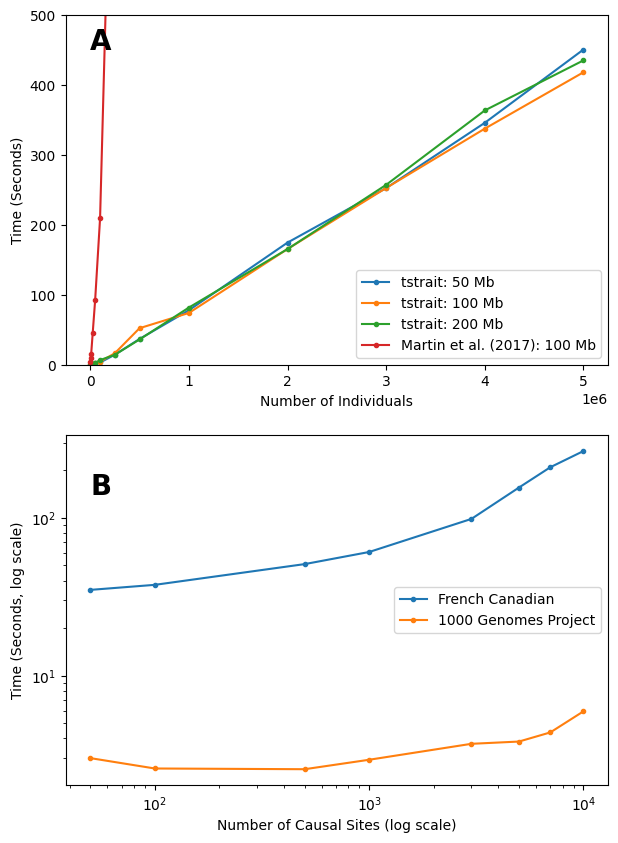
\includegraphics[width=213pt]{figure.png}
\caption{\textbf{Time taken to simulate quantitative traits.} Each point represents the mean time for 10 independent runs under different random seeds. The times reported are the total CPU time required to simulate quantitative traits on an Intel(R) Core(TM) i9-11900H CPU and 16 GB of RAM.
The trait model is a normal distribution with $\mu=0$, $\sigma^2=1$, $h^2=0.3$, and $\alpha=-1$. (A) Computational time with increasing number of individuals. The whole genome dataset from \emph{Homo sapiens} with various number of individuals and chromosome length are simulated by using \texttt{stdpopsim} \citep{adrion2020}. For each replicate of the simulation, \texttt{tstrait} is used to simulate one quantitative trait with 1000 causal sites. (B) Computational time with increasing number of causal sites on two large realistic ARGs. \texttt{tstrait} is used to simulate quantitative traits from the simulated French Canadian dataset \citep{anderson2023} and the inferred tree sequence dataset of the 1000 Genomes Project \citep{kelleher2019} with varying number of causal sites. The French Canadian dataset is downloaded from \url{https://zenodo.org/record/6839683}, and the inferred ARG from the 1000 Genomes Project is downloaded from \url{https://zenodo.org/record/3051855}. Chromosome 9 is selected for both datasets.}\label{fig:time}
\end{figure}

\section{Conclusion}

We believe that in the coming years, simulation in tree sequence encoding will attract more users in need of conducting genetic simulations with complex population structure. Multiple studies highlight the advantages of using the ARG data structure in GWAS \citep{link2023,salehi2023,zhang2023}. ARG data structure is becoming increasingly useful in genetic studies, as it is possible to accurately infer biobank-scale genealogies from sequencing data \citep{zhang2023}, and simulate large sample whole-genome sequences with spatiotemporal metadata \citep{anderson2023}. These advances in ARG presents a real opportunity for people to further understand the effects of complex population structure on quantitative traits. The \texttt{tstrait} package is an essential piece of infrastructure that lets people explore these possibilities.

\section{Competing interests}
No competing interest is declared.

\section{Acknowledgments}

We greatly acknowledge helpful discussions about quantitative trait simulation with Gregor Gorjanc. We thank Ben Haller and people in the tskit community for helpful discussions and feedback. We thank Ben Jeffery for his help with the Python package development.

\section{Funding}

D.T. is supported by the Oxford Kobe Scholarship from the University of Oxford and the Euretta J. Kellett Fellowship from Columbia University.

This work was supported by ...


%USE THE BELOW OPTIONS IN CASE YOU NEED AUTHOR YEAR FORMAT.
\bibliographystyle{abbrvnat}
\bibliography{reference}

\end{document}
